\documentclass[a4paper, 12pt]{scrartcl}
\usepackage{graphicx}
\usepackage{appendix}

% hyperref and nameref so that we can have sane internal refs
% hyperref also helps with pdf index creation
\usepackage[linkcolor={blue},citecolor={blue},urlcolor={red}]{hyperref}
\usepackage{nameref}

% Packages required to display french language characters - acute, grave,
% Guillemets, cedillas, etc.
\usepackage[utf8]{inputenc}
\usepackage[frenchb]{babel}

% Set to false for black/white printing
\hypersetup{colorlinks=true}

\title {Student Robotics 2011\\ Règlement}
\date{\today}
\setcounter{tocdepth}{1}

\begin {document}
\maketitle

\noindent Ce qui suit définit les règles du concours 2011 de Student Robotics.

\newcounter{rule}[section]
\newcommand{\rcn}{\stepcounter{rule}\arabic{section}.\arabic{rule}}
\renewcommand{\labelenumi}{\rcn}

\section {Game Rules}
\label{game-rules}

\begin{enumerate}
\item The game that will be played is called \textbf{Supermarket Sweep}.
\item The arena (see \nameref{sec:Specifications}) will contain 9 tokens (8 around the track, and 1 on the ramp).
 They will be arranged randomly, with 2 on each side as shown in \autoref{fig:arena-dim}.
 The token on the ramp --- also know as the ``\textbf{super token}'' --- will be distinguishable by a human only (by a marking on top).
\item Teams will be assigned a corner of the arena that their robot will start the game in.
 The robot must be placed within $100mm$ of both of the arena walls.
\item At the end of a match, after all tokens have settled, a team's ``\textbf{game points}'' will be calculated.
 These are used to rank teams before competition league points are awarded.
\item A token will be considered to have been collected by a robot if, at the end of the game, that token is supported by a robot.
 Tokens touching the floor or walls of the arena or ramp will not be counted.

\item The arena is considered to be split into quadrants, with the boundary lines going from corner to corner (see \autoref{fig:quadrants}).

\begin{figure}
\begin{center}
  
\includegraphics[keepaspectratio, clip, width=0.5\textwidth]{./images/quadrants.pdf}
  \caption{\label{fig:quadrants}The arena split into quadrants.
           Note that the lines won't actually exist, they are just here to illustrate.}
\end{center}
\end{figure}

\item Robots must travel in an anti-clockwise direction to gain any points.

\item Game points are awarded as follows:

\begin{itemize}
\item When a robot moves from its starting position, \textbf{1 point} is awarded.
\item When a robot enters a new quadrant\footnote{The back of the robot must be beyond the imaginary quadrant line.}, \textbf{2 points} are awarded.
\item When a robot carries any token (that includes the super token) over a quadrant boundary, \textbf{1 point} is awarded.
\item When the back of a robot passes the top of the upward-sloping section of the ramp, \textbf{3 points} are awarded.
\item When the back of a robot passes the bottom of the downward-sloping section of the ramp, \textbf{3 points} are awarded.
\item When a robot ends the game holding\footnote{To find out if a robot is holding a token, it will be lifted clear of any arena surfaces that may be supporting a token.} a normal token, \textbf{2 points} are awarded.
\item When a robot ends the game holding the super token, their \textbf{total score} for that game will be \textbf{doubled}.
\end{itemize}

\item At the end of a game, the team with the \emph{most} game points is awarded 4 points towards the competition league.
 The team with the second most is awarded 3.
 The team with the third most is awarded 2 points, and the team with the fewest game points is awarded 1 point.
 Teams whose robot was not entered into the round, or who were disqualified from the round, will be awarded no points.

\item There will be a maximum of 4 robots in a match.
\item A match lasts 180 seconds.
\item Matches are started and stopped by the Student Robotics Infrared system\footnote{The Student Robotics Infrared system is supplied as part of the kit.
 It is used for safety cut-off, start-match and stop-match signals.}.
\item Teams that do not present their robot promptly for a match will forfeit that match.
\end{enumerate}

\newpage
\section {Regulations}
\label{sec:Regulations}

\begin{enumerate}

% Overarching safety

\item All robots must be safe.

\begin{enumerate}
  \item It must not be possible to directly or indirectly injure oneself on the robot.
        Exposed sharp edges and fast moving parts, for example, will be tested using a Frankfurter sausage to simulate a finger.
        Teams are encouraged to discuss any safety concerns about their robot on the Student Robotics forums.

  \item The robot's power switch must be on the outside top of the robot and easily accessible at all times -- including throughout the game.
        This is for everyone's safety, especially your robot's.

  \item The lithium-ion polymer batteries provided in the kit must be shielded from mechanical and thermal harm.
        This includes mechanical protection from accidental impact with other robots.
        Teams found to be in violation of this rule will have their batteries confiscated until they have demonstrably rectified the identified issues.

  \item Only the power board may be connected directly to the battery.
\end{enumerate}

%% Meta

\item The Judge's decision is final.
\item Any assistance from Student Robotics volunteers is provided without guarantees.
\item Student Robotics reserves the right to examine your robot software and hardware at any time.

%% Behaviour

\item No remote control systems may be used.
\item This is a non-contact sport, but accidental bumps and scrapes are inevitable.
\item Robots must not intentionally damage anything -- including tokens, zone barriers, the arena or other robots.
      At the discretion of the judge, teams who deliberately engage in collisions or take insufficient precautions against collisions may be penalised, including disqualification from rounds and deduction of league points.
\item All kit deployed by Student Robotics remains the property of Student Robotics.
      All electronic kit \textbf{must} be returned to Student Robotics after the competition.
      \autoref{sec:kit-return} details the parts of the kit that must be returned.
      After the competition, the kit that is not specified in \autoref{sec:kit-return} becomes the property of the team.

%% Physical

\item Robots must pass an inspection by a Student Robotics Inspector before competing in a match.
      This inspector will check that the robot complies with the rules and regulations of this game, and is safe to compete (see \autoref{sec:safety-regs}).
      \textbf{Robots that have not passed inspection will not be permitted to compete}.

\item At the beginning of each match, robots must fit within a cube with $500mm$ internal sides.
      \textit{During the match}, the robot may extend beyond this size.

\item All wires connected to the robot's ground (0V line) must be black.
      Black wires \emph{must not} be used for anything else.
      It is \emph{strongly recommended} that all wiring is neat and easily removable, as this will reduce the time required to debug problems on robots
       (teams may be asked to tidy their wiring before a Student Robotics volunteer will approach any issues with their robot).

\item All electronics must be securely fixed to the robot, and should also be easily removable.

\item All robots must have mountings for the removable robot flags
      provided by Student Robotics, as described in section~\ref{sub:robot-flag}. A mounting
      must firmly hold a flag in an upright position. Flags must be mounted on the top of the robot.

\item If teams wish to use batteries other than the lithium-ion polymer batteries provided,
       then they must seek approval from Student Robotics through the Student Robotics forums first.
      Additionally, if teams wish to add systems powered by separate batteries then they must seek approval through the same channel first.

      In general, teams are encouraged to power everything off the Student Robotics supplied battery through the power board.

\item Robots may not include radio transmitters or receivers.
      In exceptional circumstances, teams may request an exemption from this rule.

\item Robots must not have any devices designed for the sole purpose of producing audible noise, with the exception of the piezoelectric buzzer on the power board.

\end{enumerate}

\newpage
\section{Specifications}
\label{sec:Specifications}

\newcounter{rulei}[subsection]
\newcommand{\rcnii}{\stepcounter{rulei}\arabic{section}.\arabic{subsection}.\arabic{rulei}}
\renewcommand{\labelenumi}{\rcnii}

\subsection{Markers}
\label{sub:markers}
The arena, tokens, slots, and robots involved in the game are labelled with \textit{libkoki} markers.
Each marker pattern encodes a number.
Each marker number is associated with a particular feature within the arena, and also has an associated size.
The marker numbers and sizes are as follows:

\begin{center}
  \begin{tabular}{lcc}
    \toprule
    \textbf{Item} & \textbf{Marker Numbers} & \textbf{Marker Size (mm)} \\
    \midrule
    Arena boundary & {} 0 -- 27 & 250 \\
    Robots & 28 -- 31 & 100 \\
    Slots & 32 -- 39 & 160 \\
    Token Top & 40 -- 43 & 160 \\
    Token Bottom & 44 -- 47 & 160 \\
    Token Side & 48 -- 51 & 160 \\
    \bottomrule
  \end{tabular}
\end{center}

Two sets of marker codes will be used: one for development purpose, and one for the competition itself.
The competition set is only to be used inside the Student Robotics arena at the Student Robotics competition.
This is so that people carrying markers past the arena do not confuse robots.
The competition codes are 100 above the development codes.
When run in competition mode (specifiable through the robot's GUI), the software provided by Student Robotics will subtract 100 from the detected marker codes, as well as ignore the development codes.

The markers can be printed on a black-and-white printer.
Marker designs can be downloaded from the documentation section of the Student Robotics website.

Unless specified otherwise, all markers described in this document are oriented vertically such that the principle corner of the marker (which is indicated by a dark grey dot in the black marker border) is on the higher edge.

\subsection{Robot Badges}
\label{sec:robot-badges}

\begin{figure}
  \centering
  
\includegraphics[width=\textwidth]{./images/robot-marker.pdf}
  \caption{An example robot badge.
           The blue areas shown are the human-compatible areas.
	   All dimensions are in millimetres.}
  \label{fig:example-badge}
\end{figure}

\begin{enumerate}
\item A ``robot badge'' is a removable identifier that will be attached to a robot throughout a match.
      It features the robot's assigned marker for the match, as well as human-compatible areas to allow spectators to easily associate a robot with its starting location.
      An example of one of these badges is shown in figure~\ref{fig:example-badge}.
      The markings in the human-compatible areas are intentionally not specified.

\item A robot must feature four of the badge mounts shown in figure~\ref{fig:badge-mounting}.
      These mounts must permit a flat $200 \times 100mm$ panel to be attached to them.
      The three areas of each mount must feature the illustrated areas of hook-type Velcro to allow this panel to be fitted.

\item The four badge mounts must be on the exterior of the robot, parallel with the vertical plane, and should be perpendicular to each other about the vertical axis\footnote{Teams can apply for a team-specific rule alteration to the required number of badges.
      Clear justification must be provided by the team with such a request.}
      The orientation of the badge mounts is unimportant, but teams are encouraged to position them horizontally as shown in figure~\ref{fig:example-badge}.

\item The mapping between a given robot and its robot badge is as follows:

\begin{center}
  \begin{tabular}{cc}
    \toprule
    \textbf{Corner} & \textbf{Marker Number} \\
    \midrule
    0 & 28 \\
    1 & 29 \\
    2 & 30 \\
    3 & 31 \\
    \bottomrule
  \end{tabular}
\end{center}

\begin{figure}
  \centering
  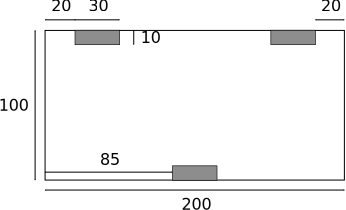
\includegraphics[width=\textwidth]{./images/badge-mounting.pdf}
  \caption{The dimensions of the required robot badge mountings.
           The shaded areas are hook-type Velcro.
           All dimensions are in millimetres.}
  \label{fig:badge-mounting}
\end{figure}

\end{enumerate}

\subsection{Arena}
\label{sub:arena}
\begin{enumerate}
\item The match arena floor, overall, is an $8m \times 8m$ square, as shown in figure~\ref{fig:arena-dim}.
      The tolerance of these two dimensions is $\pm0.25m$.

\begin{figure}
  \centering
  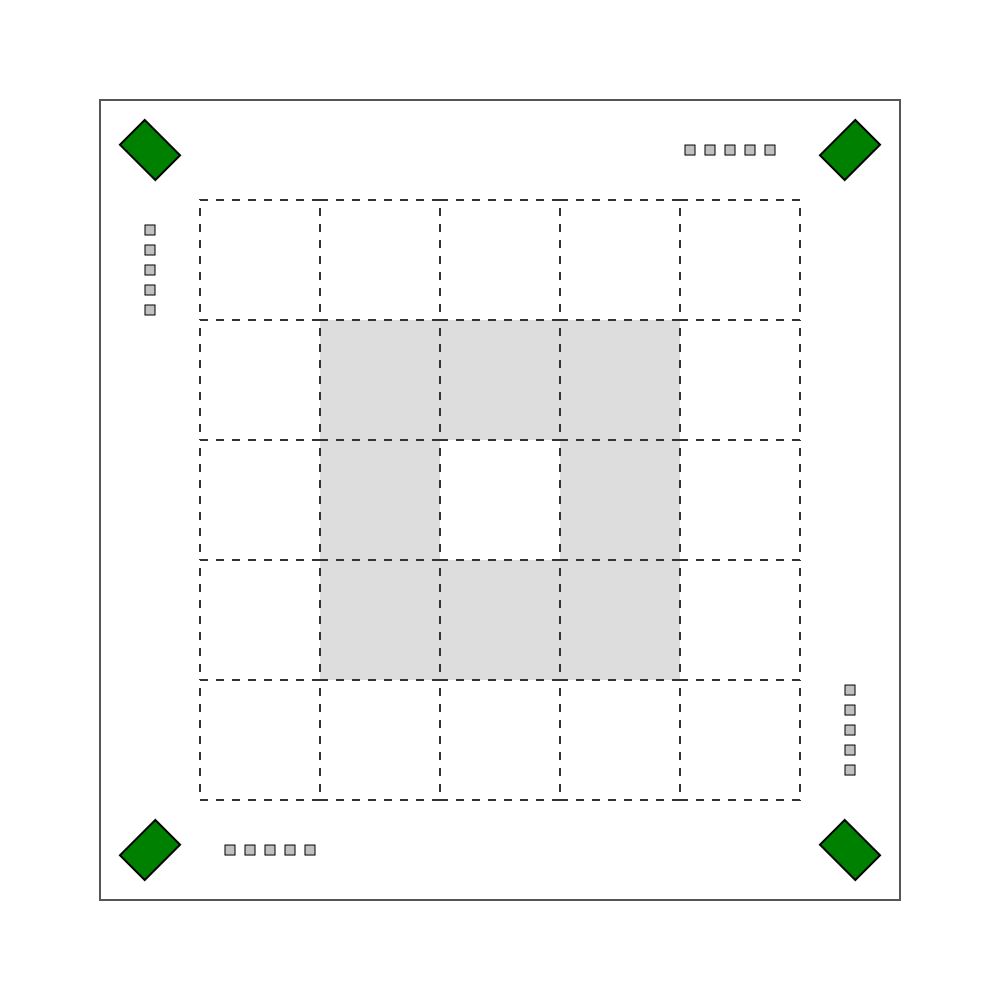
\includegraphics[width=\textwidth]{./images/arena.pdf}
  \caption{\label{fig:arena-dim}A bird's-eye view of the arena. All dimensions are in millimetres.}
\end{figure}

\item The floor of the arena is carpeted with blue carpet tiles.

\item The arena walls are $600\pm30mm$ high, the interior surfaces of which are white plastic-coated hardboard.

\begin{figure}
  \centering
  
\includegraphics[width=\textwidth]{./images/sidewall.pdf}
  \caption{Seven $250mm$ wide markers are spaced evenly along each $8m$ arena wall.
           The markers are placed $50mm$ above the floor.
	   All dimensions are in millimetres.}
  \label{fig:arena-wall}
\end{figure}

\begin{figure}
  \centering
  
\includegraphics[width=0.5\textwidth]{./images/arena-markers.pdf}
  \caption{Twenty eight arena wall markers are positioned around the perimeter of the arena with the marker codes incrementing in an anti-clockwise fashion.
           Eight slot markers are incremented from number 32, in an anti-clockwise fashion around the zones.
           The corners are counted in a clockwise fashion, with corner 0 being the corner closest to arena marker 0.}
  \label{fig:arena-zones}
\end{figure}

\item Each wall of the arena features seven $250mm$ libkoki markers.
      Figure~\ref{fig:arena-wall} shows the positioning of these markers, whilst figure~\ref{fig:arena-zones} shows the numbering of these markers.

\item Each robot will be assigned a corner at the start of every match to indicate its starting position.
      Corner starting positions are $1000 \pm 20mm$ square and will be marked by $25mm$ paper-based masking tape.
      The mapping of these corner numbers in the arena is shown in figure~\ref{fig:arena-zones}.

\item Student Robotics reserves the right to have up to three match officials in the arena during games.

\end{enumerate}


\subsection{Zones}
\label{sub:Zones}

\begin{figure}
  \centering
  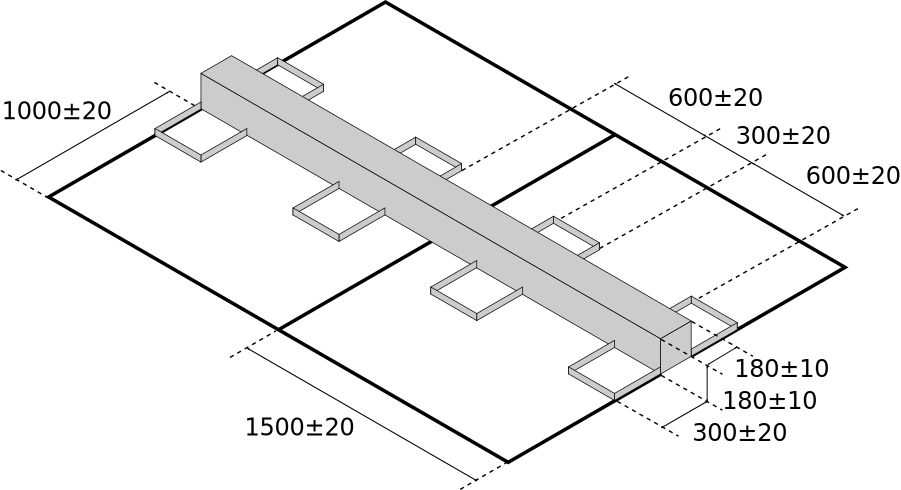
\includegraphics[width=\textwidth]{./images/slots-zones.pdf}
  \caption{The arena contains four zones, each $1500 \pm 20mm$ wide and $1000 \pm 20mm$ deep.
           The rectangle described by the four zones is split in two by a $180 \pm 10mm$ high, $180 \pm 10mm$ deep zone wall.
           Eight $25 \pm 5mm$ high slots---two in each zone---are attached to the zone wall.
           All dimensions are in millimetres.}
  \label{fig:slots-zones}
\end{figure}

\begin{enumerate}
\item There are four zones in the centre of the arena.
      The arrangement of these zones can be seen in figure~\ref{fig:arena-dim}, and is shown in more detail in figure~\ref{fig:slots-zones}.

\item Each zone is $1500mm$ wide and $1000mm$ deep and is  marked with $25mm$ wide paper-based masking tape.

\item A single $180 \pm 10mm$ high, $180 \pm 10mm$ deep wall splits the four zones in two.
      The position of the wall can be seen in figure~\ref{fig:slots-zones}.
\end{enumerate}


\subsection{Slots}
\label{sub:slots}

\begin{enumerate}
\item There are eight slots in the arena.
      Two slots appear in each zone, as shown in figure~\ref{fig:slots-zones}.

\item Each slot is identified by a unique $160mm$ libkoki marker (see section~\ref{sub:markers}).
      Slot markers are affixed to the zone wall, each centered in their corresponding slots, and $20 \pm 5mm$ above the floor.
      Figure~\ref{fig:arena-zones} shows which markers identify which slots.

\item Slots are attached to the zone wall.

\item The boundary of each slot is constructed using square cross-sectioned wood with a side length of $25 \pm 5mm$.

\item Externally, each slot is $300 \pm 20mm$ wide and $300 \pm 20mm$ deep.

\end{enumerate}


\subsection{Tokens}
\label{sub:Tokens}
\begin{enumerate}
\item Tokens are cubic corrugated cardboard boxes with side $200 \pm 15 mm$.
      \emph{Each team's kit contains two of these.}

\item Each robot has eight identical tokens associated with it, two in each corner.

\item A token for a given robot will be labelled with three distinct $160mm$ libkoki markers: one for the top, one for the bottom, and four identical markers for the remaining sides.

\item Token side markers are oriented such that the top left corner of each marker (identified by a small grey dot) is affixed to the top left of a token's side face, with the top and bottom markers affixed accordingly.

\item Tokens will be styled to match the human-compatible area of the robot badges on their associated robot, allowing spectators to follow game play.
      See section~\ref{sec:robot-badges}.

\item The mapping between a given robot and its associated markers is as follows:

\begin{center}
  \begin{tabular}{cccc}
    \toprule
    \textbf{Corner} & \textbf{Top Marker} & \textbf{Bottom Marker} & \textbf{Side Markers} \\
    \midrule
    0 & 40 & 44 & 48 \\
    1 & 41 & 45 & 49 \\
    2 & 42 & 46 & 50 \\
    3 & 43 & 47 & 51 \\
    \bottomrule
  \end{tabular}
\end{center}

\item Tokens will initially be positioned to the left and right of the robot as shown in figure~\ref{fig:token-position}.

\begin{figure}
  \centering
  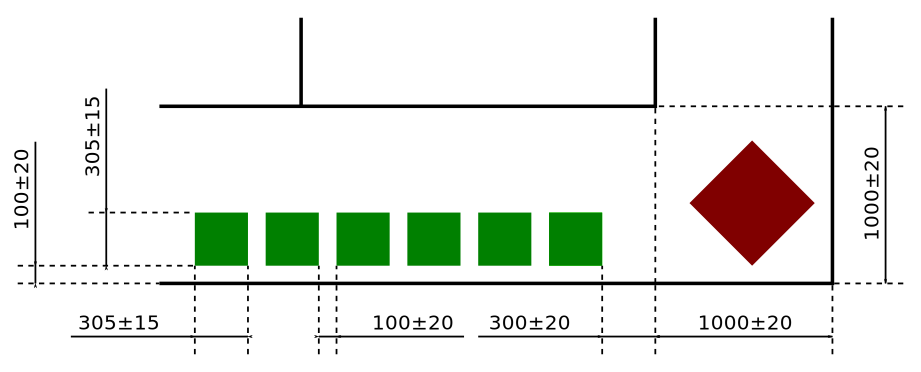
\includegraphics[width=\textwidth]{./images/token-position.pdf}
  \caption{Two perpendicular rows of four $200 \pm 15mm$ wide tokens are spaced evenly $300 \pm 20mm$ to the left and right of the robot's starting boundaries, along the arena walls.
    The tokens are placed $200 \pm 20mm$ away from each other, and $100 \pm 20mm$ from the arena wall.
           All dimensions are in millimetres.}
  \label{fig:token-position}
\end{figure}

\end{enumerate}

\clearpage

\newpage
\section {Awards}
\label{sec:Awards}

\subsection{Main Competition Awards}
Prizes will be awarded to the teams that are placed highest at the end of the competition.
The teams in $1^{st}$, $2^{nd}$ and $3^{rd}$ place will receive awards.

\subsection{Rookie Award}
The Rookie Award will be awarded to the rookie
team\footnote{A rookie team is one from a school, college or independent group that hasn't competed in Student Robotics before.}\addtocounter{footnote}{-1}\addtocounter{Hfootnote}{-1}
 that places highest in the league.

\subsection{Committee Award}
The Committee Award will be given to the team that displays the most extraordinary ingenuity in the design of their robot.
It will not be awarded for complexity of design, rather the implementation of a simple and elegant solution to a problem.

\subsection{Robot and Team Image}
The team that presents their robot and themselves in what is judged to be the most outstanding way will receive this award.

\subsection{First Robot Movement}
The first rookie team\footnotemark{} that demonstrates a moving robot to the community will be awarded with an edible prize at the final competition.
\begin{enumerate}
\item The robot movement must be controlled by software running on the Student Robotics kit.
\item The robot must move 2 metres, pause for 2 seconds, turn 180$^\circ$ ($\pm20^\circ$), return to its starting position ($\pm0.5m$), and come to a halt without interference.
\item This must be demonstrated by a video on the web (e.g. on YouTube, flickr, etc.) and linking to this video from a post on the Student Robotics forum.
\end{enumerate}

\subsection{Online Presence}
The team that is judged to have the best online presence will be awarded with an edible prize at the final competition.
 An online presence is a publicly available set of web pages detailing the team's progress, it can involve blog posts, pictures and videos of the team and the robot.
 \emph{Hint: Useful sites include blogger.com, wordpress.com, flickr.com and youtube.com}
\begin{enumerate}
\item When detailing activities online do not post any private information concerning yourself or others.
\item Notify Student Robotics about the location of your online materials on the Student Robotics forums.
\end{enumerate}


\renewcommand{\labelenumi}{\rcn}

\section{Clarifications}
Requêtes de clarification des règles peuvent être envoyées à \href{mailto:info@studentrobotics.org}{\nolinkurl{info@studentrobotics.org}}. Requêtes qui sont reçues en moins d'un mois avant le concours sont peu probables d'être adressées.
Les modifications suivantes ont été apportées aux règles depuis leurs diffusion initiale.

\newpage
\appendix
\appendixpage
\addappheadtotoc
\section {Return of Kit}
\label{sec:kit-return}

Each team is responsible for ensuring that they return these items from their kit.

\subsection {Items to be Returned}

\begin{tabular}{ll}
 \toprule
 \textbf{Item} & \textbf{Quantity} \\
 \midrule
 18l Really Useful Box & 1 \\

 %% SR-specific stuff
 Power Board & 1 \\
 Brain Board (Odroid U3) & 1 \\
 Motor Board & 2 \\
 Servo Board & 1 \\
 Ruggeduino & 1 \\
 Screw Shield & 2 \\

 %% USB stuff
 USB Hub & 2 \\
 USB Memory Stick & 1 \\
 USB WiFi Adapter & 1 \\
 Webcam (C500 or C270) & 1 \\
 USB A to USB B lead & 3 \\
 USB A to USB Micro-B lead & 5 \\

 %% Battery stuff
 Lithium Polymer Battery & 2 \\
 Battery Charger (IMAX B6 or HobbyKing E4) & 1 \\
 Charger Power Supply and Mains Cable & 1 \\
 Battery charging bag & 1 \\

 %% Misc. stuff
 7.5mm Green Camcon plugs & 10 \\
 5mm Green Camcon plugs & 7 \\
 3.81mm Green Camcon plug & 1 \\
 ODROID Power Cable & 1 \\
 Screwdriver & 1 \\
 \bottomrule
\end{tabular}

\subsection {When and How to Return Kit}

The kit must be returned by the end of the competition.
If you wish to keep the kit beyond the competition, then this \textbf{must} be arranged with us,
 before the 22\textsuperscript{nd} of March \sryear, via email to \href{mailto:teams@studentrobotics.org}{\nolinkurl{info@studentrobotics.org}}.


\end {document}
